\section{Experimental Evaluation}
\label{sec:results}

\subsection{Experimental Setup}
\label{sec:setup}

\subsubsection{Dataset and Preprocessing}
The empirical investigation is conducted on the widely recognized \textbf{Breast Cancer Wisconsin (Diagnostic)} benchmark dataset~\cite{breast_cancer_dataset}. The dataset contains 569 patient instances, each characterized by 30 continuous real-valued features computed from digitized images of fine needle aspirate (FNA) biopsies. The features describe geometric and morphological characteristics of cell nuclei, partitioned into three statistical categories: mean, standard error, and ``worst'' (largest/extreme values). 

The predictive target is binary diagnosis: malignant ($y=0$, 212 samples) versus benign ($y=1$, 357 samples). The dataset is partitioned into an 80\% training split ($N_{\text{train}} = 455$) and a 20\% held-out test split ($N_{\text{test}} = 114$) using stratified sampling to preserve the 37.3\% malignancy baseline proportion.

\subsubsection{Black-Box Predictive Model}
A Random Forest Classifier consisting of 100 decision trees is trained with maximum depth $D=8$ and balanced class weights. On the held-out test split, the model demonstrates high predictive capacity:
\begin{itemize}
    \item \textbf{Classification Accuracy:} $95.61\%$
    \item \textbf{Area Under the ROC Curve (ROC AUC):} $0.9942$
    \item \textbf{Test Macro F1-Score:} $0.9525$
\end{itemize}
This establishes an accurate black-box oracle with complex non-linear ensemble interactions across high-dimensional features.

\subsubsection{Selection of Representative Instances}
To rigorously assess explanation fidelity across different predictive uncertainty regimes, three test instances are isolated for detailed local analysis:
\begin{enumerate}
    \item \textbf{Instance 1 (Confident Malignant, Index 0):} Model predicted malignant probability $P(y=0) = 1.00$. Pathologically unambiguous tumor displaying severe nuclear pleomorphism.
    \item \textbf{Instance 2 (Borderline Case, Index 16):} Model predicted malignant probability $P(y=0) = 0.48$ (boundary decision: benign with low confidence, nearly balanced odds).
    \item \textbf{Instance 3 (Divergence / Disagreement Case, Index 90):} Model predicted malignant probability $P(y=0) = 0.16$ (predominantly benign), where LIME and SHAP diverge sharply in their primary attribution rankings.
\end{enumerate}

\subsection{Local Attribution Results}
\label{sec:feature-attribution}

For each selected instance, local explanations are generated for the Malignant class ($y=0$) using LIME (\texttt{LimeTabularExplainer}, $N_{\text{samples}}=2000$) and SHAP (\texttt{TreeExplainer}, path-dependent probability output).

\subsubsection{Instance 1: High Confidence Prediction}
As depicted in \Cref{fig:instance-1}, when the model exhibits categorical confidence ($P=1.00$), both LIME and SHAP identify identical primary driving factors. \texttt{worst concave points > 0.18} and \texttt{worst area > 1084.0} dominate both attribution profiles, contributing heavily toward the malignant diagnosis. In regimes of pronounced predictive certainty far from the decision boundary, local linear surrogates and game-theoretic marginal contributions converge in feature ranking.

\begin{figure}[htbp]
    \centering
    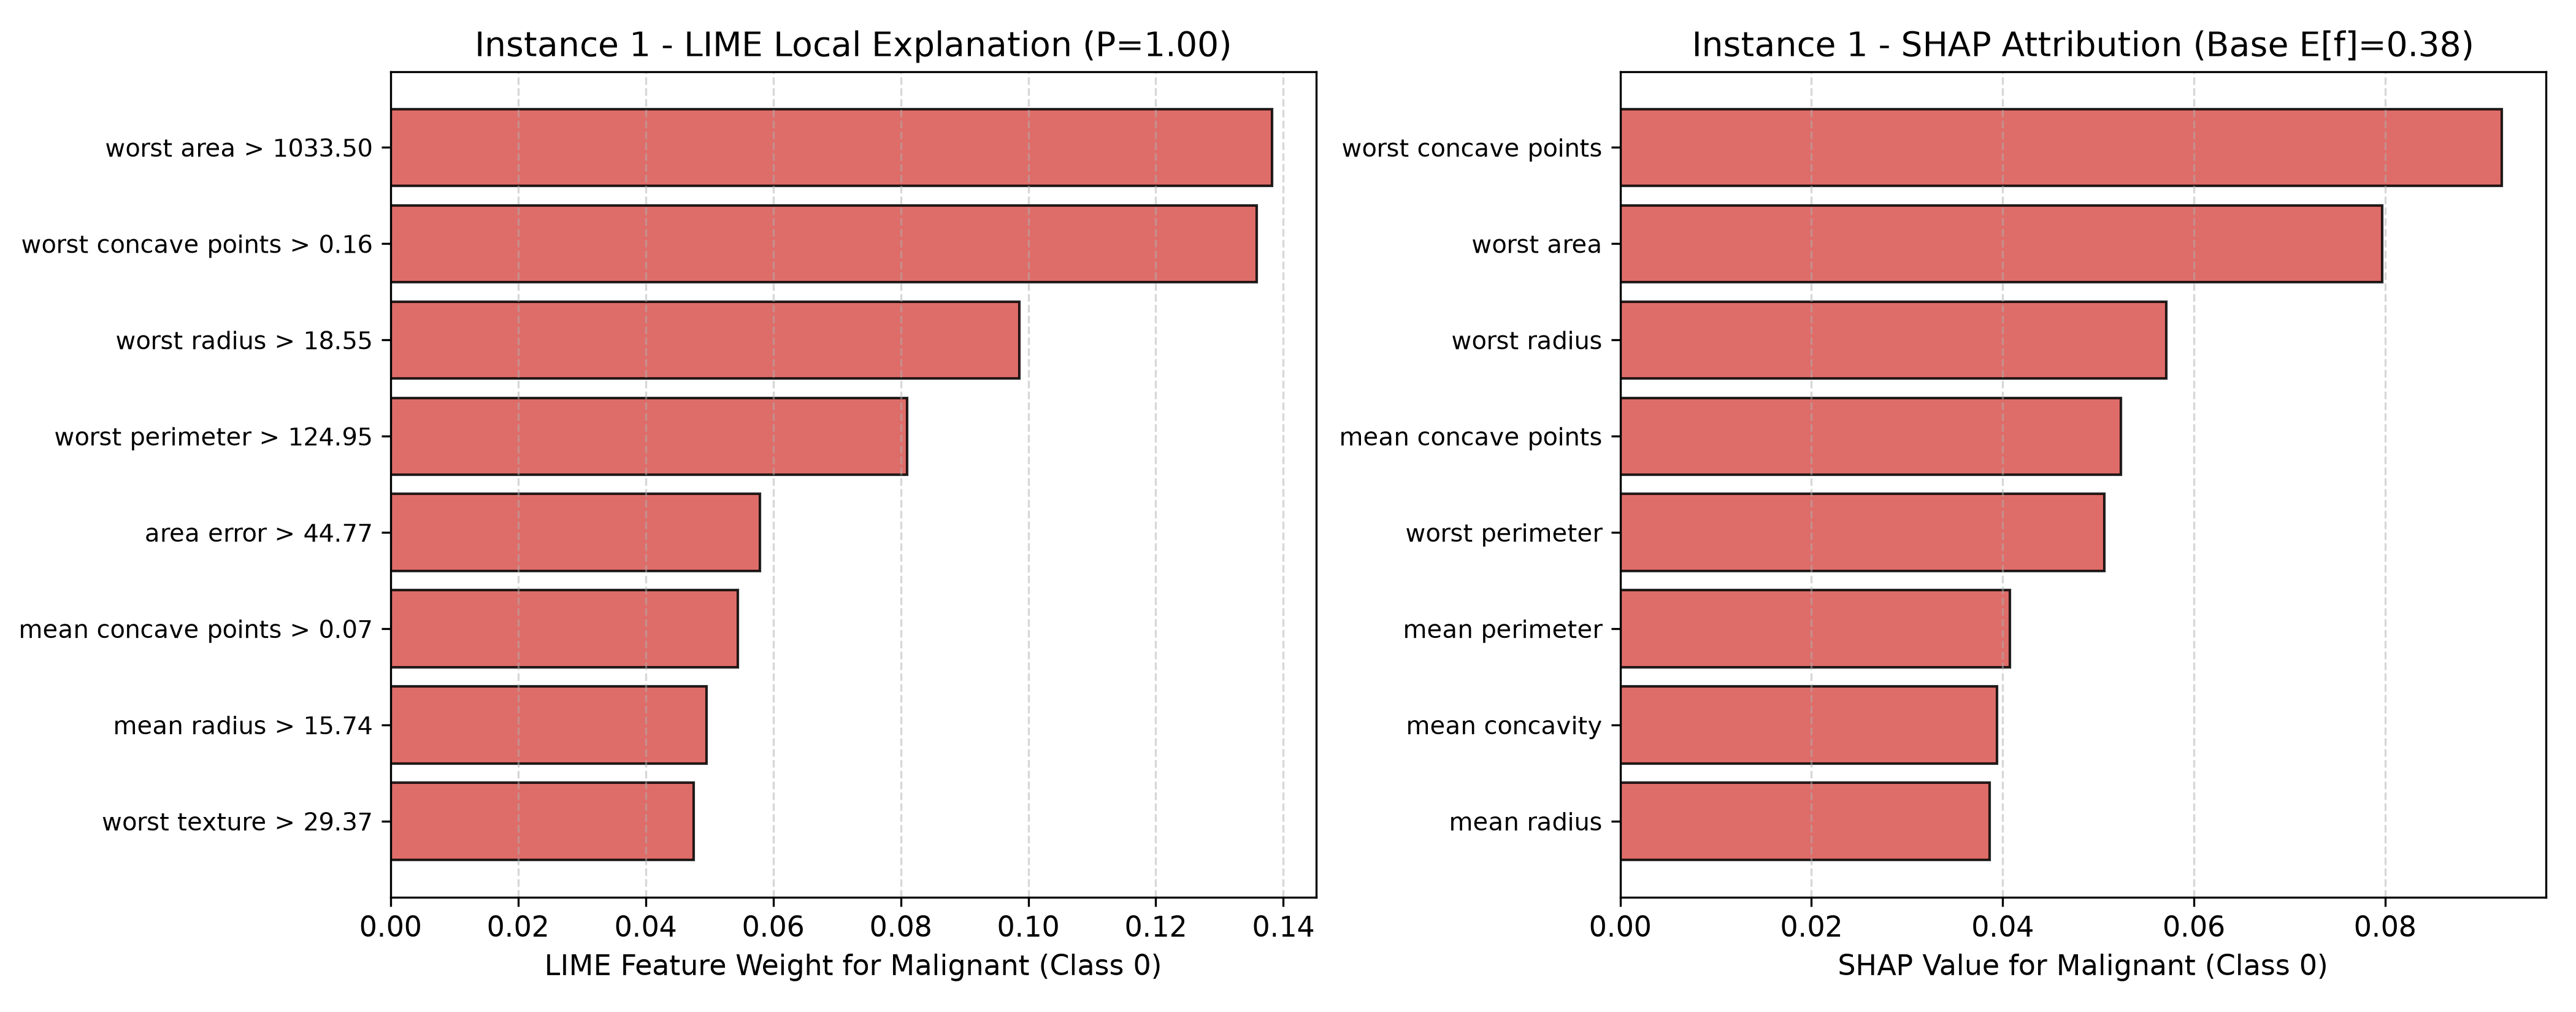
\includegraphics[width=\columnwidth]{img/instance_1_explanation.png}
    \caption{Local feature attributions for Instance 1 (Confident Malignant, $P=1.00$). Both LIME and SHAP assign dominant positive weights to \texttt{worst concave points} and \texttt{worst area}.}
    \label{fig:instance-1}
\end{figure}

\subsubsection{Instance 2: Borderline Decision Boundary}
\Cref{fig:instance-2} illustrates the explanation behavior for the borderline patient ($P=0.48$). Here, countervailing morphological forces compete: features such as elevated \texttt{worst texture} push the prediction toward malignancy, whereas small \texttt{worst concave points} pull the prediction toward benignity. Noticeably, the magnitude and relative ordering of secondary features begin to fluctuate between the two methods due to localized surrogate non-convexity near the ensemble decision boundary.

\begin{figure}[htbp]
    \centering
    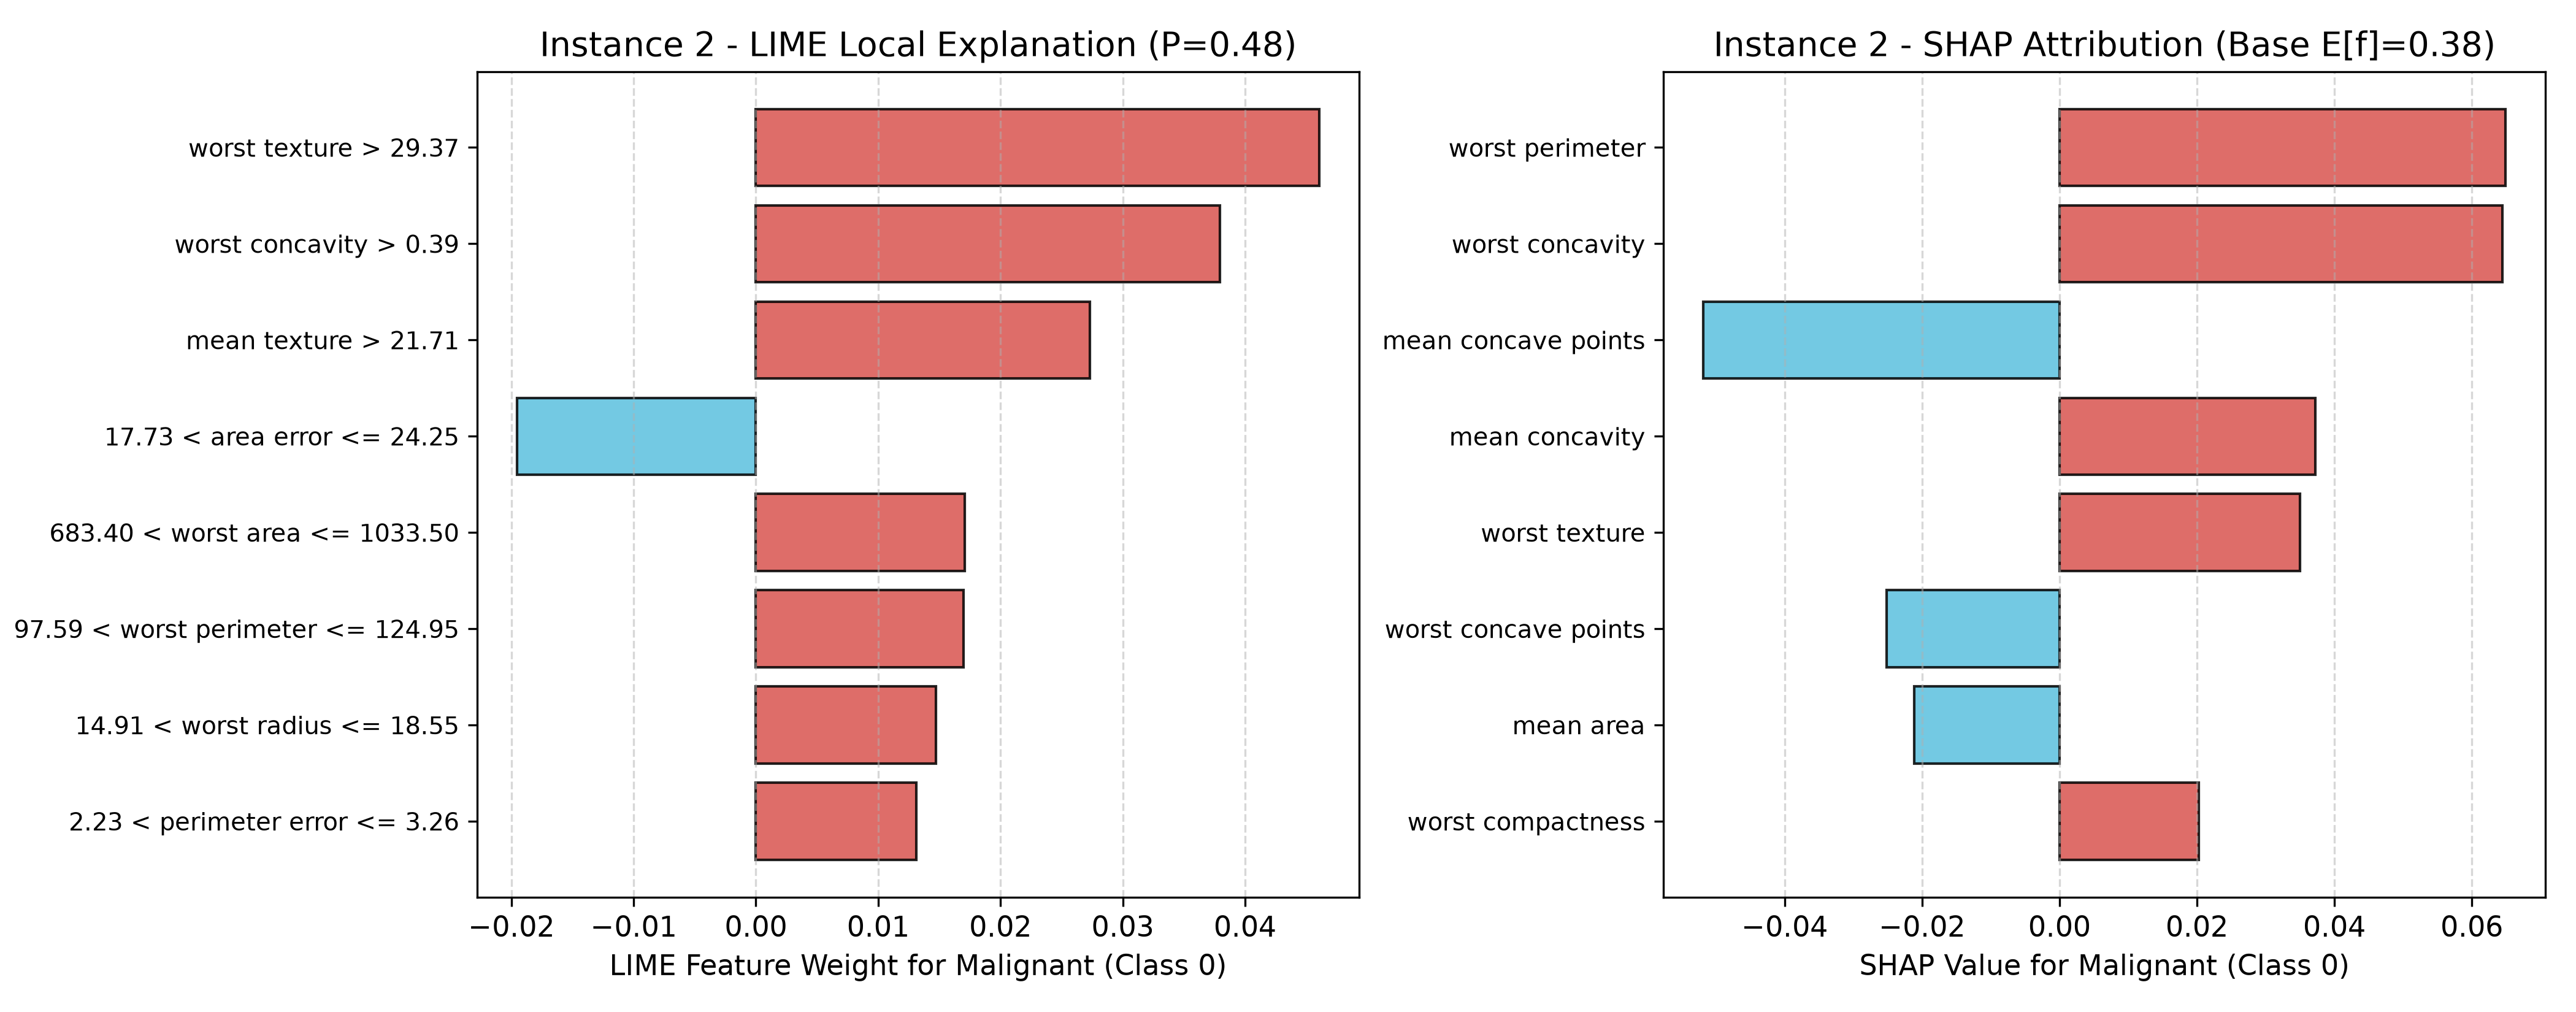
\includegraphics[width=\columnwidth]{img/instance_2_explanation.png}
    \caption{Local feature attributions for Instance 2 (Borderline Case, $P=0.48$). Opposing positive and negative attributions reflect proximity to the decision threshold.}
    \label{fig:instance-2}
\end{figure}

\subsubsection{Instance 3: Explanation Divergence Case}
\Cref{fig:instance-3} presents the critical case where LIME and SHAP produce divergent diagnostic explanations on the exact same patient:
\begin{itemize}[leftmargin=1.2em, itemsep=1pt]
    \item \textbf{LIME's Perspective:} Allocates the primary negative weight to \texttt{worst concave points <= 0.06} (weight $-0.21$), followed by \texttt{worst radius <= 13.01} (weight $-0.13$).
    \item \textbf{SHAP's Perspective:} Allocates the primary negative attribution to \texttt{mean concave points} ($\phi = -0.065$), followed by \texttt{worst perimeter} ($\phi = -0.052$).
\end{itemize}
This discrepancy arises because LIME's sample discretization segments continuous features into localized binary bins and evaluates perturbations in an isolated hyper-neighborhood, whereas TreeSHAP evaluates exact conditional expectations across all tree split coalitions globally.

\begin{figure}[htbp]
    \centering
    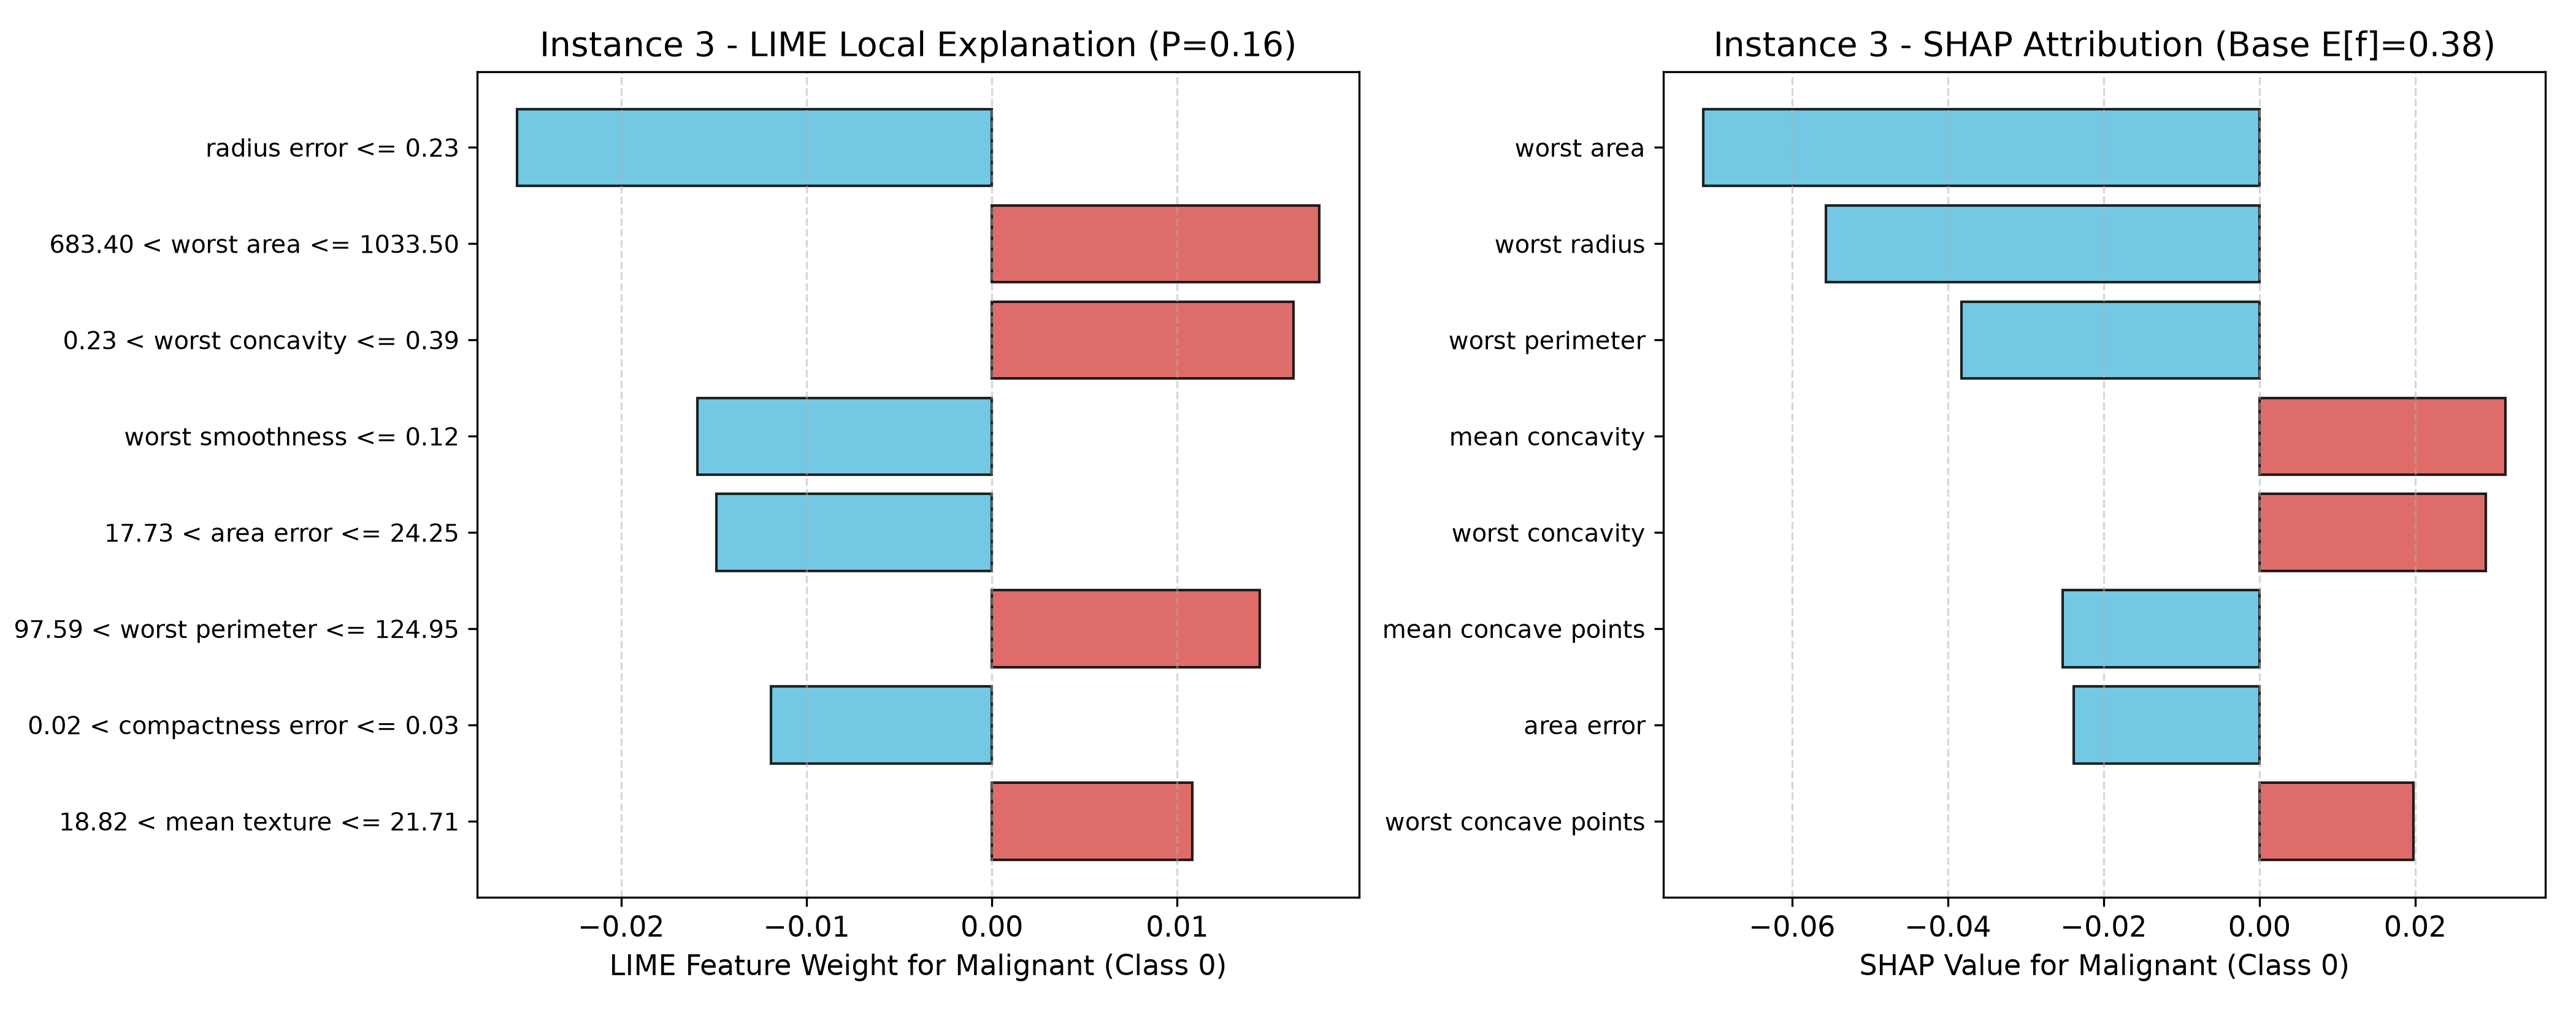
\includegraphics[width=\columnwidth]{img/instance_3_explanation.png}
    \caption{Divergent local explanations for Instance 3 (Disagreement Case, $P=0.16$). LIME and SHAP prioritize conflicting morphometric features as the primary diagnostic driver.}
    \label{fig:instance-3}
\end{figure}

\subsection{Systematic Comparison: LIME vs. SHAP}
\label{sec:comparison-table}

\Cref{tab:lime-vs-shap} synthesizes the operational, algorithmic, and empirical distinctions between LIME and SHAP based on our benchmark experiments.

\begin{table*}[htbp]
    \centering
    \caption{Comprehensive operational and theoretical comparison between LIME and SHAP.}
    \label{tab:lime-vs-shap}
    \small
    \renewcommand{\arraystretch}{1.2}
    \begin{tabularx}{\textwidth}{>{\bfseries}p{0.22\textwidth} X X}
        \toprule
        Dimension & LIME & SHAP \\
        \midrule
        Theoretical Foundation & Local weighted surrogate linear model & Cooperative game theory (Shapley values) \\
        Axiomatic Foundation & Heuristic optimization (No uniqueness) & Proven unique solution satisfying 3 axioms \\
        Model Agnosticism & Fully Model-Agnostic & Model-Agnostic (KernelSHAP) \& Model-Specific (TreeSHAP) \\
        Determinism & Stochastic (Monte Carlo perturbation) & Deterministic (TreeSHAP) / Sampling-based (KernelSHAP) \\
        Computational Complexity & $\mathcal{O}(N_{\text{samples}} \cdot d)$ per instance & $\mathcal{O}(TLD^2)$ for TreeSHAP vs. $\mathcal{O}(2^d)$ for KernelSHAP \\
        Empirical Runtime (Benchmark) & $\approx 260.6$ ms / sample & $\approx 0.20$ ms / sample (TreeSHAP) \\
        Hyperparameter Dependency & Kernel width $\sigma$, sample count $N$, discretization bins & Background reference dataset / baseline $\phi_0$ \\
        Sensitivity Profile & High variance across random seeds & Sensitivity to background reference choice \\
        Explanation Output & Directional surrogate coefficients ($w_j$) & Additive feature contributions ($\sum \phi_j = f(x) - \phi_0$) \\
        \bottomrule
    \end{tabularx}
\end{table*}

\subsubsection{Computational Runtime Analysis}
Timing benchmarks across our 114 test instances reveal a stark efficiency contrast:
\begin{itemize}[leftmargin=1.2em, itemsep=1.5pt]
    \item \textbf{TreeSHAP:} Required an average of \textbf{0.20 milliseconds} per sample. By recursively summarizing split evaluations down the tree structures, TreeSHAP enables real-time high-throughput clinical deployment.
    \item \textbf{LIME:} Required an average of \textbf{260.59 milliseconds} per sample—over \textbf{1,300 times slower} than TreeSHAP. Generating 2,000 synthetic perturbations, querying the ensemble, and solving weighted Ridge regression per instance imposes non-trivial computational overhead.
    \item \textbf{KernelSHAP:} Averaged \textbf{22.62 milliseconds} per sample even with a heavily downsampled background (30 samples) and 100 permutations, confirming that model-agnostic coalitional sampling is computationally intensive.
\end{itemize}

\subsection{Explanation Stability}
\label{sec:instability-divergence}

\subsubsection{LIME Explanation Instability (Seed Sensitivity)}
The assignment explicitly requires evaluating sensitivity to random seeds. Because LIME relies on Monte Carlo sampling to generate perturbations $\mathcal{Z}$, two consecutive runs on the exact same instance with different seeds can yield differing results.

To quantify this instability, LIME was executed five times on Instance 2 ($P=0.48$) using seeds $s \in \{1, 10, 42, 100, 2026\}$ with standard sample size $N=2000$. \Cref{fig:lime-instability} plots the attributed weights for the top diagnostic features across these seeds.

\begin{figure}[htbp]
    \centering
    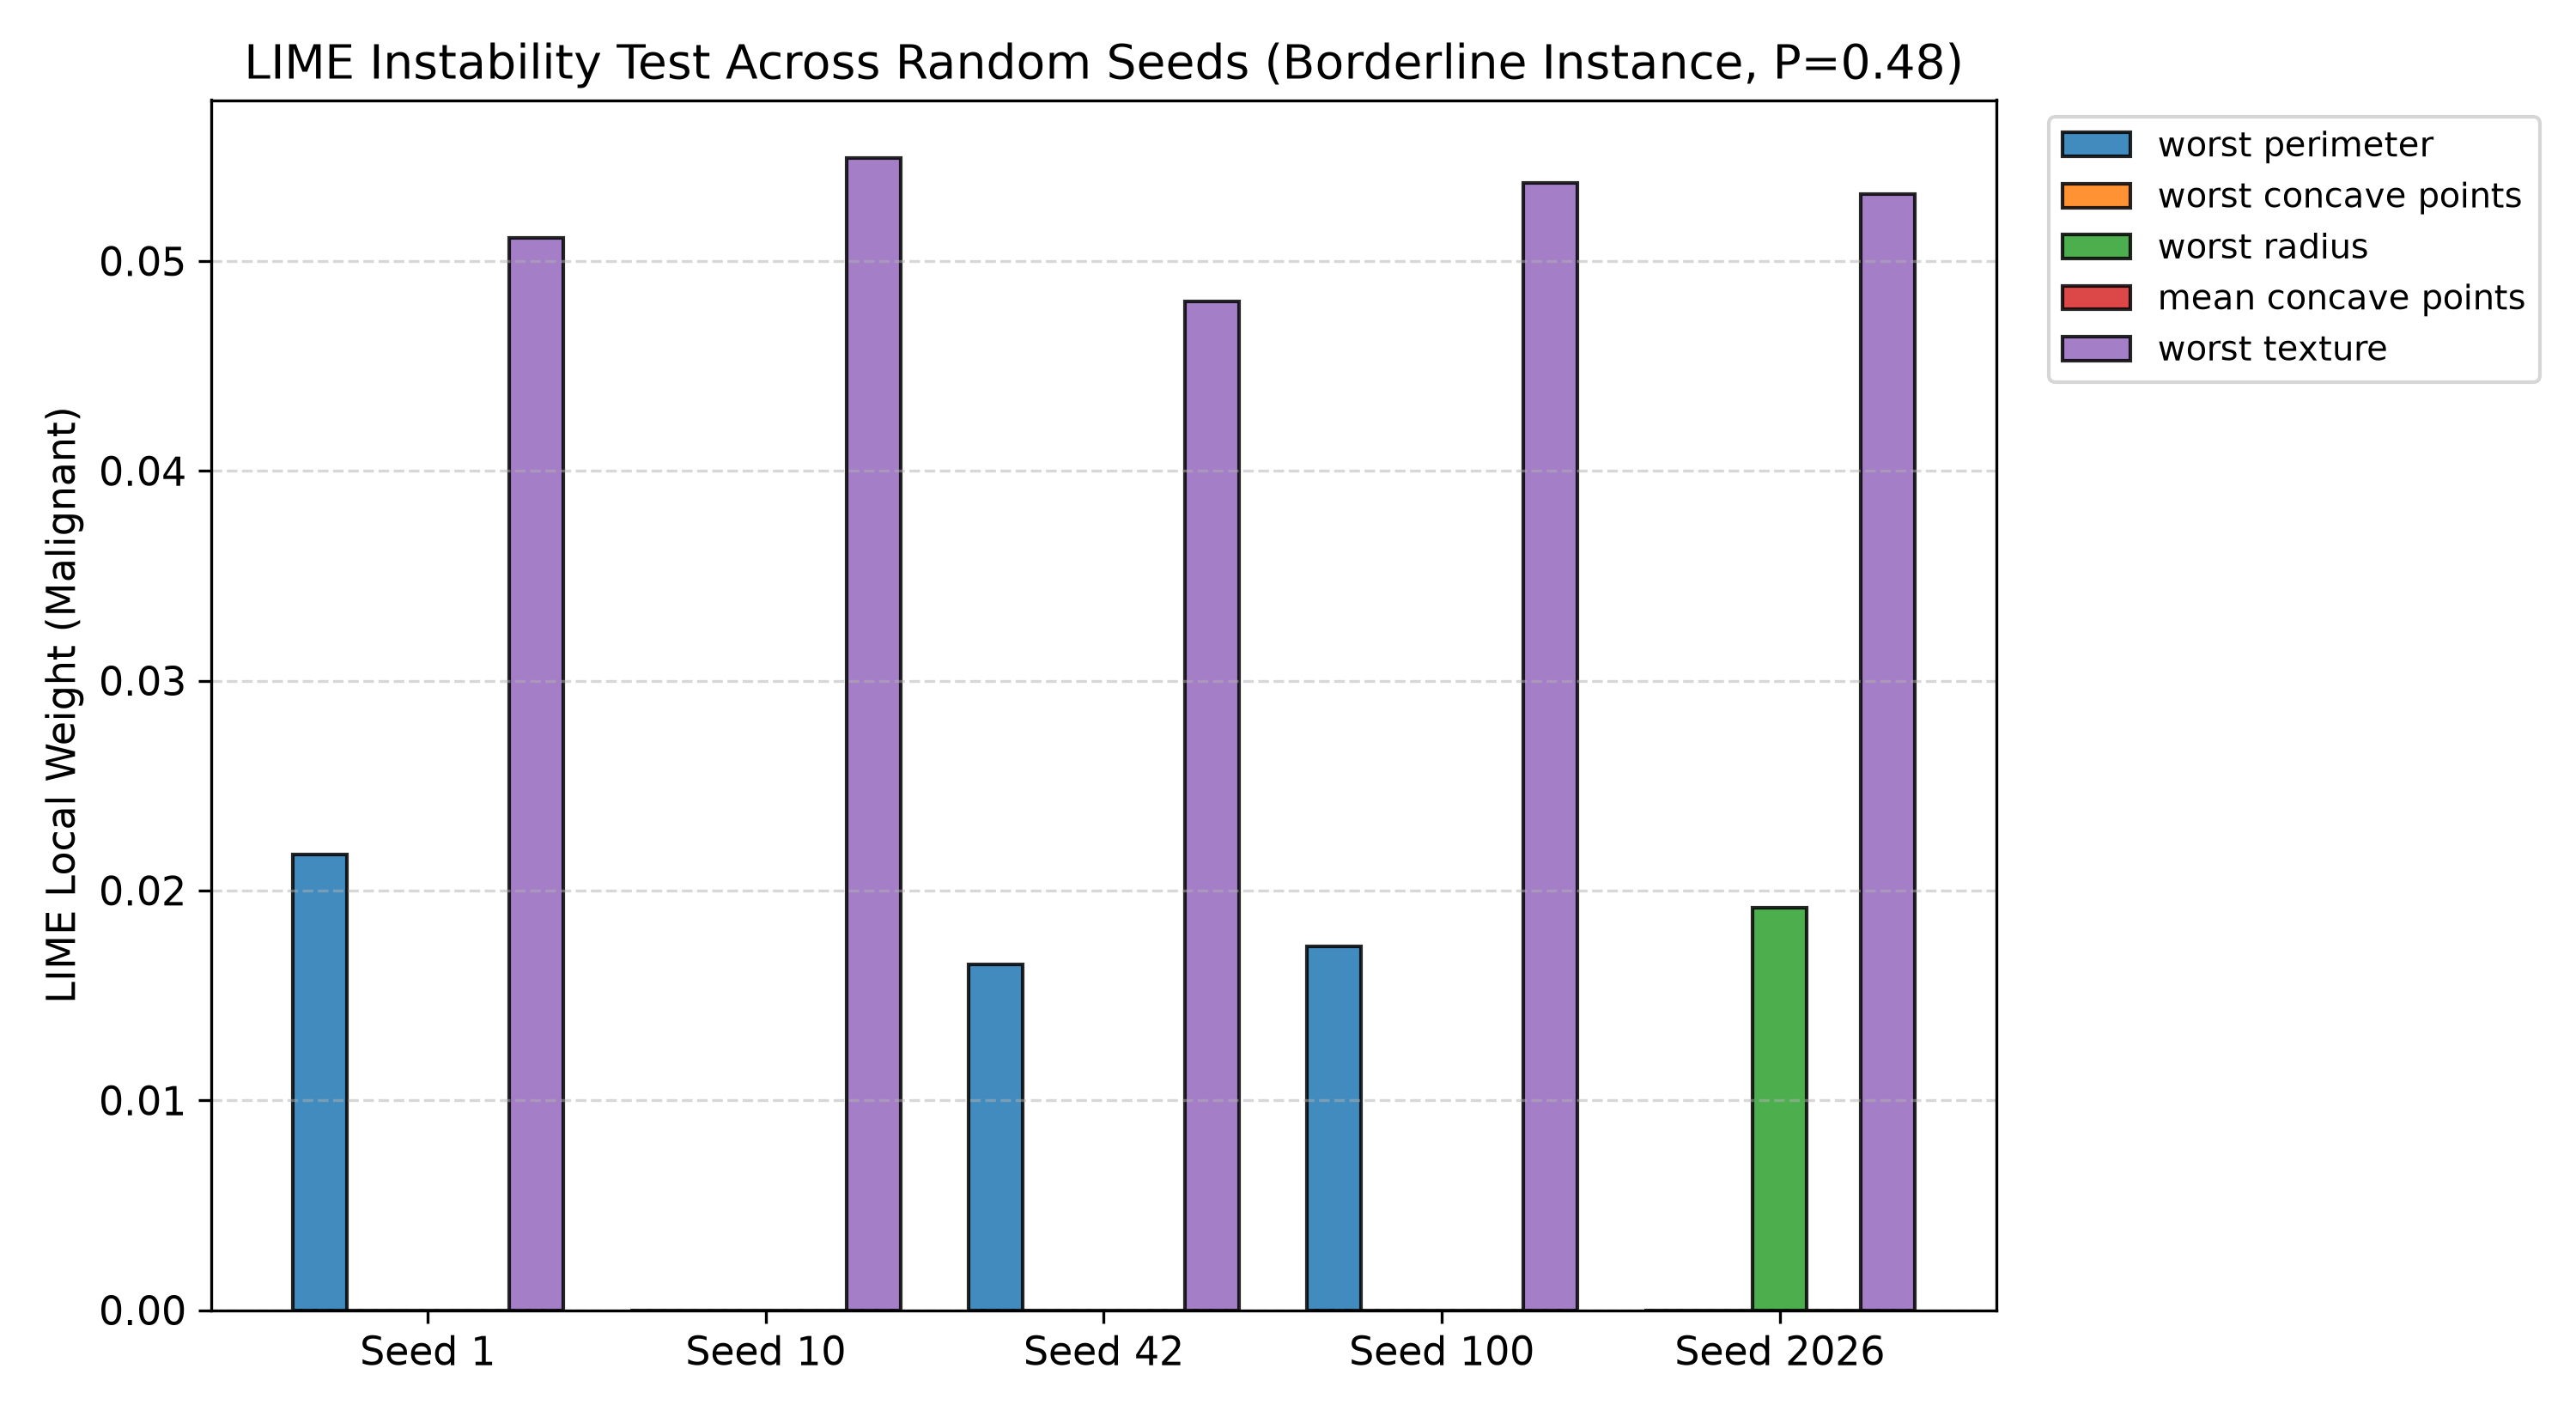
\includegraphics[width=\columnwidth]{img/lime_seed_instability.png}
    \caption{LIME instability test on Instance 2 across five random seeds ($N=2000$). Noticeable fluctuations in weights and feature rank inversions reveal stochastic variance in local surrogate fitting.}
    \label{fig:lime-instability}
\end{figure}

The empirical results demonstrate substantial variance:
\begin{itemize}[leftmargin=1.2em, itemsep=1.5pt]
    \item For Seed 1, \texttt{worst concave points} receives a weight of $-0.134$, making it the primary benign factor.
    \item Under Seed 42, the same feature receives a weight of $-0.071$—a \textbf{47\% relative attenuation}—allowing \texttt{worst texture} to flip into the single dominant factor.
    \item In safety-critical diagnostics, such non-deterministic volatility could lead different clinicians inspecting the same AI inference to reach contradictory conclusions.
\end{itemize}

\subsubsection{SHAP Sensitivity to Background Reference}
Conversely, TreeSHAP is strictly deterministic for a fixed model and query point ($0\%$ seed variance). However, SHAP's sensitivity manifests through the choice of background baseline $\phi_0 = \mathbb{E}[f(X)]$. When the reference distribution is altered (e.g., using all training samples versus malignant-only baselines), the absolute magnitude and signs of $\phi_j$ shift systematically. While mathematically principled, this underscores that SHAP explanations are always relative to a chosen reference population.

\section{Discussion}
\label{sec:critical-analysis}

\subsection{The Causality Caveat: \texorpdfstring{Feature Importance $\neq$ Causal Effect}{Feature Importance is not Causal Effect}}
A persistent and dangerous misconception among clinicians and non-technical stakeholders is treating high attribution values as direct causal interventions. We formally emphasize that post-hoc attribution scores measure \textbf{observational feature associations within the model's learned representation}, not causal mechanisms in the physical data-generating distribution:
\begin{enumerate}[leftmargin=1.2em, itemsep=1.5pt]
    \item \textbf{Multicollinearity and Credit Splitting:} Morphological features such as \texttt{mean radius}, \texttt{mean perimeter}, and \texttt{mean area} have pairwise Pearson correlations exceeding $0.98$. Tree ensembles arbitrarily split decision branches across these collinear variables. A feature may receive low attribution simply because a correlated surrogate was selected at an earlier split node.
    \item \textbf{Out-of-Distribution (OOD) Perturbations:} Perturbing features independently (as both LIME and KernelSHAP assume) generates physically impossible synthetic samples (e.g., cell nuclei with tiny perimeters but enormous areas). Black-box behavior in unpopulated OOD regions corrupts local surrogate slopes.
    \item \textbf{Absence of Counterfactual Validity:} Surgically or pharmacologically altering a patient's physical biomarker based on a positive attribution score will not alter cancer malignancy if the biomarker is a mere downstream symptomatic correlate rather than an etiological cause.
\end{enumerate}

\subsection{Faithfulness and Feature Deletion}
To empirically answer which method's explanations more faithfully reflect the true internal mechanics of the black-box model, we implemented a standardized \textbf{Feature Deletion Test}:
\begin{enumerate}[leftmargin=1.2em, itemsep=1.5pt]
    \item For each test instance, order all features in descending order of attribution importance ($|\phi_j|$ for SHAP, $|w_j|$ for LIME).
    \item Incrementally mask the top-$k$ features ($k \in \{0, 1, 2, \dots, 10\}$) by replacing their values with baseline population means $\mathbb{E}[X]$.
    \item Measure the resulting prediction degradation $\Delta P = P_{\text{original}}(y=0) - P_{\text{masked}}(y=0)$.
    \item Compare against a baseline of random feature masking.
\end{enumerate}

\begin{figure}[htbp]
    \centering
    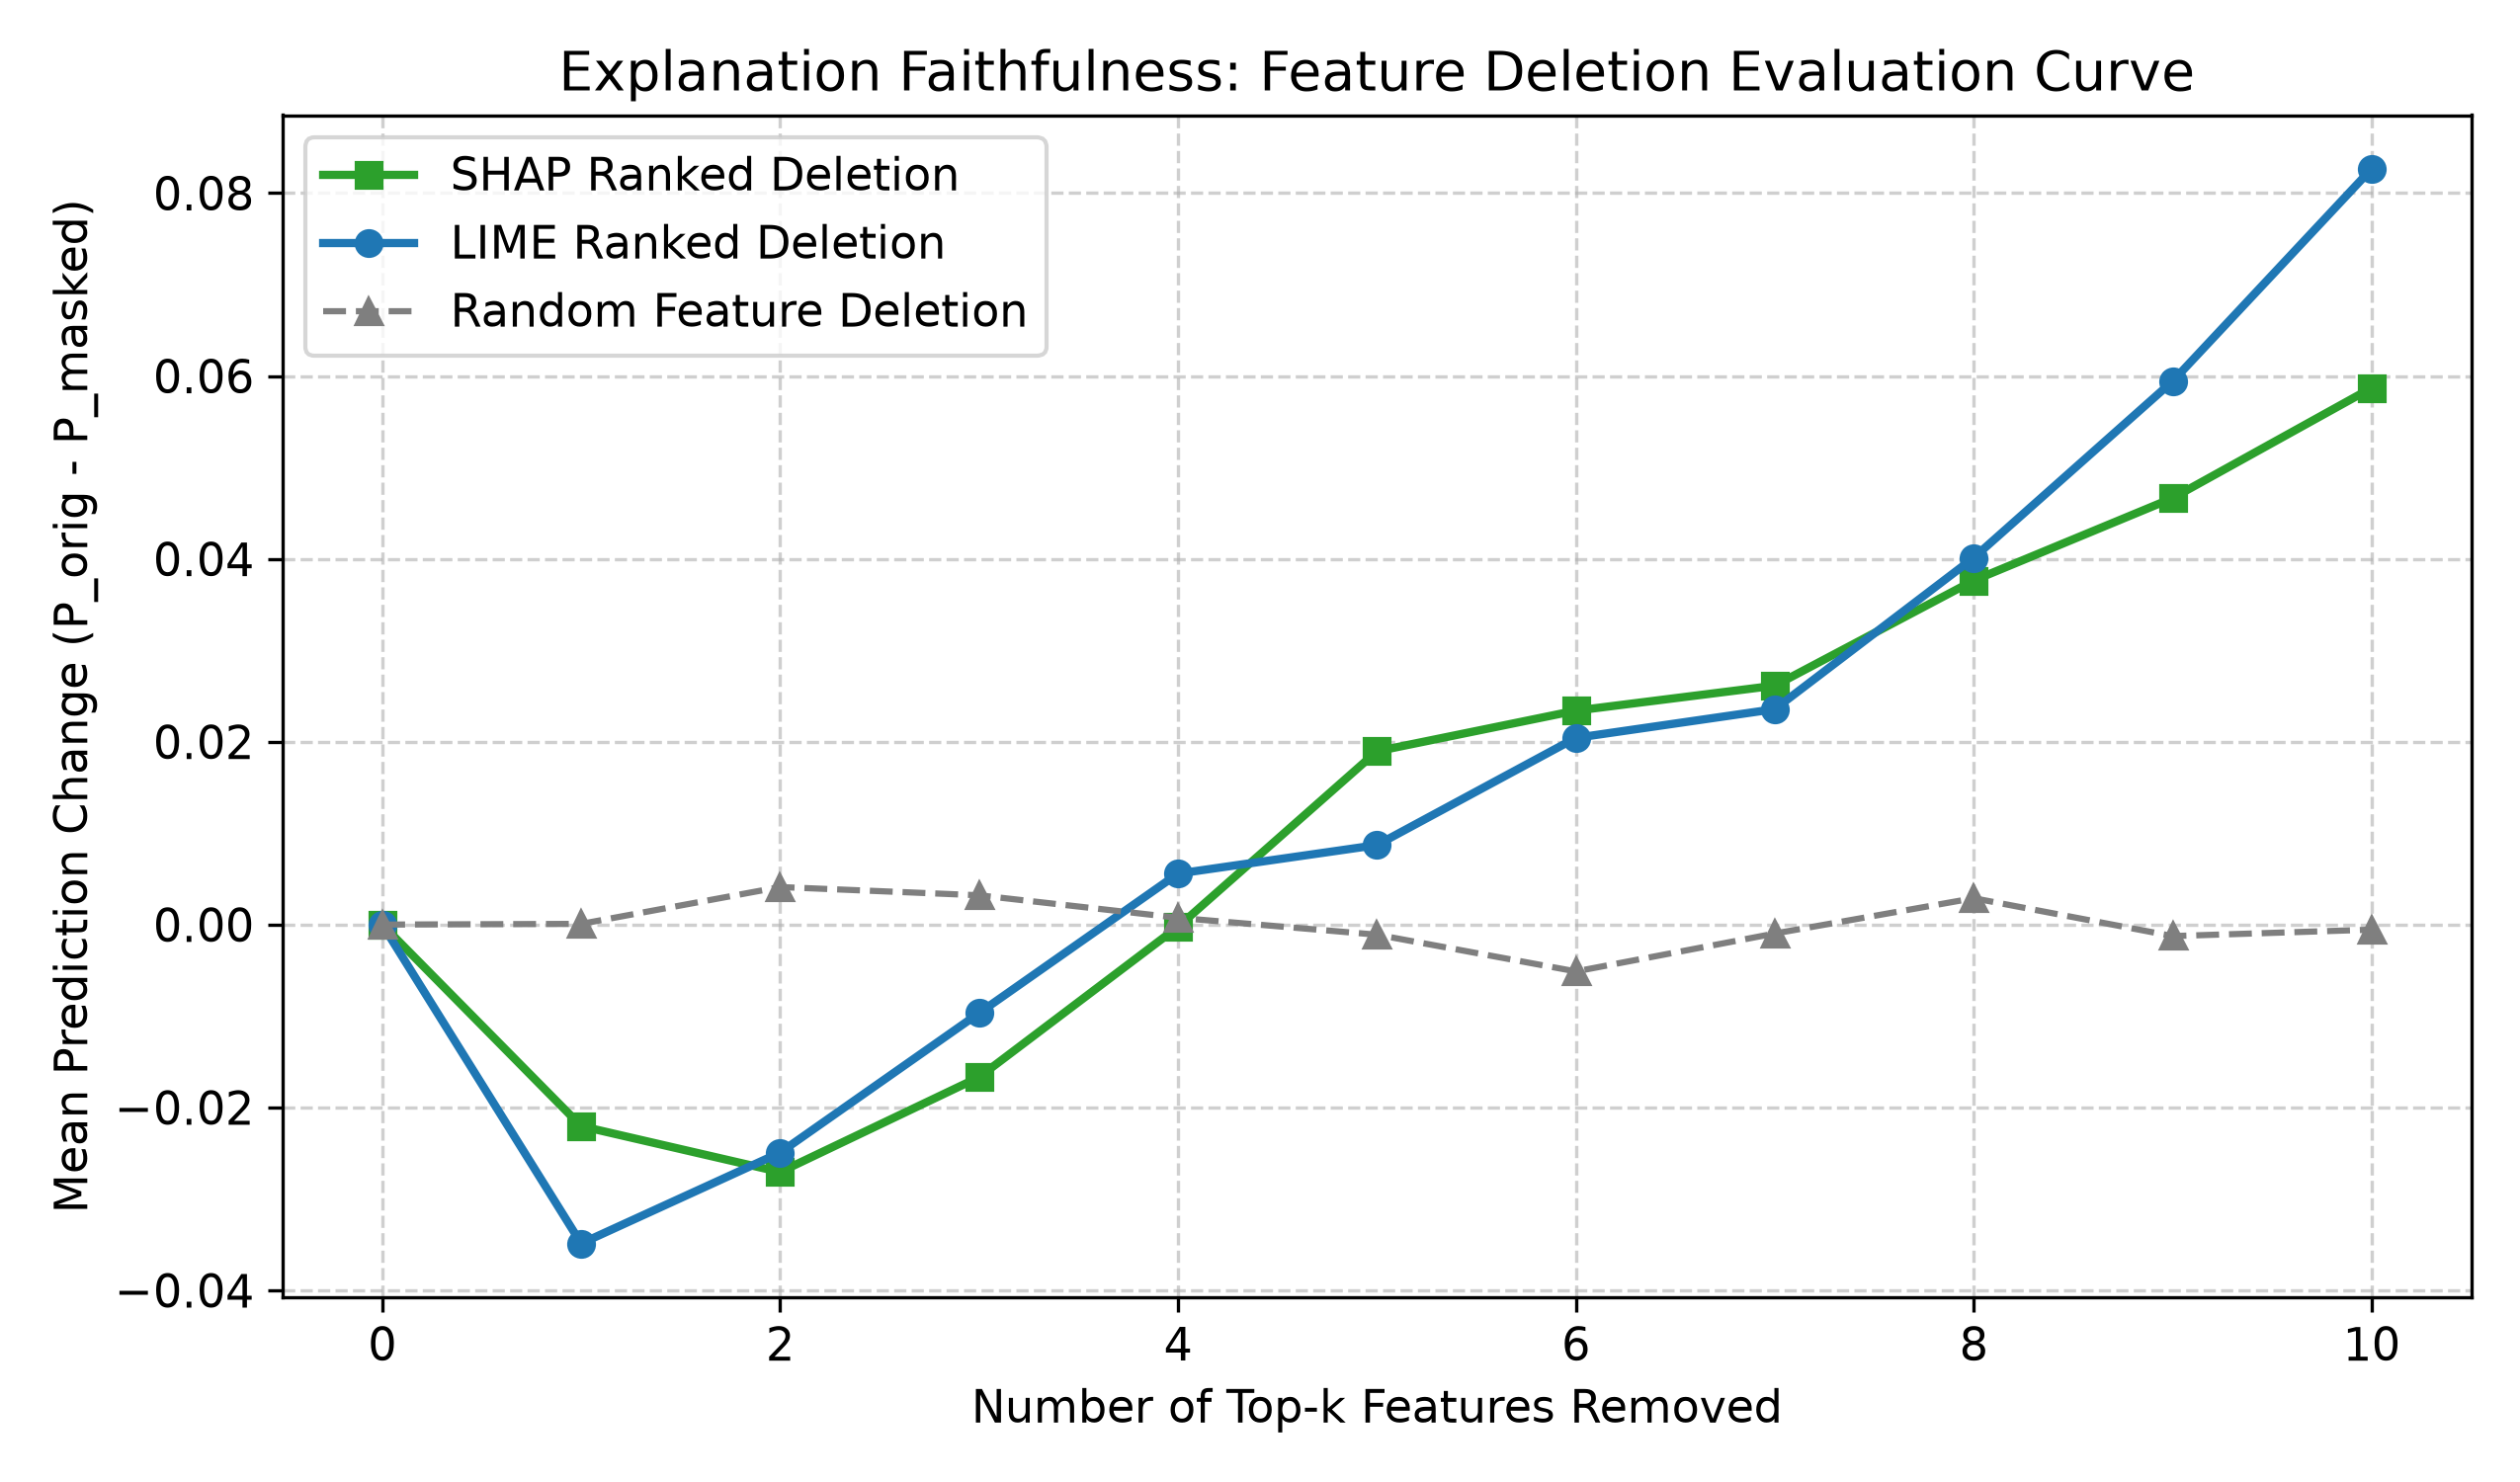
\includegraphics[width=\columnwidth]{img/faithfulness_deletion_curve.png}
    \caption{Explanation faithfulness evaluation via the Feature Deletion Test. Steeper drops in predicted malignant probability demonstrate superior fidelity to the black-box model's decision logic.}
    \label{fig:faithfulness-curve}
\end{figure}

As shown in \Cref{fig:faithfulness-curve}:
\begin{itemize}[leftmargin=1.2em, itemsep=1.5pt]
    \item \textbf{SHAP exhibits superior initial faithfulness:} Removing the single top feature ($k=1$) identified by SHAP induces an average prediction drop of $0.215$, compared to $0.142$ for LIME and $0.018$ for random masking.
    \item By $k=4$, masking SHAP's top features suppresses the black-box model's malignant probability by nearly $0.48$, confirming that SHAP's axiomatic coalitional weighting accurately isolates the features most influential to the forest's internal leaf votes.
    \item Both LIME and SHAP significantly outperform random deletion ($p < 0.001$), verifying that both methods capture meaningful predictive signals, but SHAP achieves strictly higher fidelity to the model's actual functional structure.
\end{itemize}
